\chapter{Complex numbers}

\section{Complex arithmetic}

Complex numbers can be thought of as points on the $xy$ plane. The
point $(x,y)$, thought of as a complex number, is written $x+iy$ (or
$x+jy$ if you are an electrical engineer).  The $i$ stands for an 
``imaginary" quantity such that $i^2 =-1$. 
If $z=x+iy$ then $x$ is
called the real part of $z$ and $y$ is called the imaginary part of
$z$.

Complex numbers are added just as if they were vectors in two
dimensions.  If $z=x+iy$ and $w=s+it$, then
\[
z+w=(x+iy) + (s+it) = (x+s) + i(y+t)
\]

To multiply two complex numbers, just remember that $i^2=-1$. So if
$z=x+iy$ and $w=s+it$, then
\[
zw=(x+iy)(s+it)=xs+i^2ytr +iys + ixt = (xs-yt) + i(xt+ys)
\]
The modulus of a complex number, denoted $|z|$ is simply the length of
the corresponding vector in two dimensions. If $z=x+iy$
\[
|z| = |x+iy|=\sqrt{x^2+y^2}
\]
An important property is
\[
|zw|=|z||w|
\]
just like for real numbers. 

The complex conjugate of a complex number $z$, denoted $\bar z$, is
the reflection of $z$ across the $x$ axis (also called the real axis). Thus
$\overline{x+iy}=x-iy$.  Thus complex conjugate is obtained by
changing all the $i$'s to $-i$'s.  We have
\[
\overline{zw}=\bar z \bar w
\]
and
\[
z\bar z= |z|^2
\]
This last equality is useful for simplifying fractions of complex
numbers by turning the denominator into a real number, since
\[
{{z}\over{w}} =  {{z\bar w}\over{|w|^2}}
\]
For example, to simplify $(1+i)/(1-i)$ we can write
\[
{{1+i}\over{1-i}} = {{(1+i)^2}\over{(1-i)(1+i)}}
   ={{1-1+2i}\over{2}}=i
\]
A complex number $z$ is real (i.e. the $y$ part in $x+iy$ is zero)
whenever $\bar z = z$. We also have the following formulas for the
real and imaginary part. If $z=x +i y$ then $x = (z+\bar z)/2$ and $y
= (z-\bar z)/(2i)$

Complex numbers are indispensable in many practical calculations. We
will discuss complex exponentials when we talk about differential
equations.  The reason why we are interested in them now is the
following fact:

\begin{theorem}
If we use complex numbers, every polynomial can be completely
factored.
{\rm 
In other words, given a polynomial $\lambda^n + a_{n-1} \lambda^{n-1} + \cdots
+ a_1\lambda + a_0$, there exist (possibly complex) numbers $r_1, r_2, \ldots,
r_n$ such that
\[
\lambda^n + a_{n-1} \lambda^{n-1} + \cdots
+ a_1\lambda + a_0 = (\lambda-r_1) (\lambda-r_2)\cdots(\lambda-r_n)
\]
The numbers $r_1$ are the values of $\lambda$ for which the polynomial
is zero.}
\end{theorem}

So for example the polynomial $\lambda^2+1$ has no real roots, since
there is no real number $\lambda$ for which it is zero. However there
are two complex roots, $\pm i$ and
\[
\lambda^2+1 = (\lambda + i)(\lambda - i)
\]
Of course, actually finding the roots of a high degree polynomial is
difficult.  Here are some points to keep in mind.

You can always find the roots of a quadratic polynomial using the
quadratic formula. In other words, the roots of $a\lambda^2 + b\lambda
+ c$ are
\[
{{-b \pm\sqrt{b^2-4ac}}\over{2a}}
\]
If the quantity inside the square root is negative, then the roots are
complex. So, for example the roots of $\lambda^2 + \lambda + 1$ are
\[
{{-1 \pm\sqrt{1^2-4}}\over{2}} = {{-1 \pm\sqrt{-3}}\over{2}}
= {{-1 \pm\sqrt{-1}\sqrt{3}}\over{2}}={{-1}\over{2}} \pm i
{{\sqrt{3}}\over{2}}. 
\]

\section{Complex matrices and linear systems} 

Determinants can be computed using basic arithmetic operations. Also, linear systems van be solved and matrix inverses found by applying basic arithmetic operations in Gaussian elimination. Having learned the arithmetic of complex numbers, we can apply it to finding determinants and inverses of matrices with complex entries (complex matrices) and solutions of complex linear systems. 

\subsection{Determinants of complex matrices} 

The determinant of a square matrix with complex entries is calculated in the same way as for a real matrix. As in the real case, a complex matrix is invertible if and only if its determinant is nonzero. 

\begin{example}
\label{ex:5det2} 
Calculate the determinant of 
\[
{\bf A} = \left[ \begin{array}{cc} 1+i & 2 \\ 3 & 1-2i \end{array} \right]
\] 
Using the same formula as for real matrices we compute 
\[
\det {\bf A} = (1+i)(1-2i) - 6  = -3-i.
\]
Since the determinant is not zero, $\bf A$ is invertible. We will find find the unique solution of a system with this coefficient matrix in Example~\ref{ex:5nonhom} and its inverse in Example~\ref{ex:5inverse} below. 
\end{example} 

\begin{example}
\label{ex:5det3} 
Calculate the determinant of 
\[
{\bf A} = \left[ \begin{array}{ccc} i & 0 & 3 \\ 1 & i & -1 \\ 0 & 1 & 3+i \end{array} \right]
\]
We compute 
\[
\det {\bf A} = i \left[ i (3+i) +1 \right] + 3 = -3 +3 = 0.
\]
In this example, $\bf A$ is not invertible and so has nontrivial homogeneous solutions. We will find these homogeneous solutions in Example \ref{ex:5homogeneous} below. 
\end{example}

\subsection{Homogeneous complex linear systems}

Homogeneous linear systems with complex coefficients have solutions that can be found after Gaussian elimination as was done for real systems in Chapter 3. 

\begin{example}
Find the complex numbers $x_1$, $x_2$ and $x_3$ that satisfy 
\begin{eqnarray} 
(1+i) x_1 + 2x_2 -3i x_3 & = & 0 \\
(1-i)x_1 +3x_2 + (1+i) x_3 & = & 0 
\end{eqnarray} 
Note that both right hand side values above are zero: this defines a homogeneous system. Remember that there is always at least one solution with all variables equal to zero. In this example, there will be an infinite number of solutions. We can write this system in an augmented matrix:
\[
\left[ \begin{array}{ccc|c} 1+i & 2 & -3i & 0 \\ 1-i & 3 & 1+i & 0 \end{array} \right]
\]
However, just like real homogeneous systems, we can just remember the zero right hand sides (which will stay zero during the elimination process) and write 
\begin{eqnarray}
\nonumber
\left[ \begin{array}{ccc} 1+i & 2 & -3i \\ 1-i & 3 & 1+i \end{array} \right] & \sim & 
\left[ \begin{array}{ccc} 1 & 1-i & -\frac{3}{2} - \frac{3}{2} i  \\ 0 & 3+2i  & 4+i \end{array} \right]
\begin{array}{c} (1) \div (1+i) \\ (2) - (1-i) ({\rm new}1) \end{array} \\
\label{eq:complexh}
& \sim & 
\left[ \begin{array}{ccc} 1 & 0 & -\frac{57}{26} - \frac{1}{26} i  \\ 0 & 1  & \frac{14}{13} - \frac{5}{13} i \end{array} \right]
\begin{array}{c} (1) - (1-i) ({\rm new}2) \\ (2) \div (3+2i) \end{array} 
\end{eqnarray} 
The final line (\ref{eq:complexh}) above is the homogeneous system in reduced row echelon form. It can be seen that $x_3$ is not determined. It is a free variable which we will denote by $t$, a complex parameter. From the second row of (\ref{eq:complexh}) 
\[
x_2 = -(\frac{14}{13} - \frac{5}{13}i) t 
\]
and from the first row of (\ref{eq:complexh}) 
\[
x_1 = -(-\frac{57}{26} - \frac{1}{26}i) t 
\]
or summarizing 
\[
{\bf x} = \left(  \frac{57}{26} + \frac{1}{26}i, -\frac{14}{13} + \frac{5}{13}i, 1\right) t 
\]
is a parametric form of all of the solutions to the system with $t$ any complex number.
\end{example} 

\begin{example}
\label{ex:5homogeneous} 
Find a nontrivial solution to the homogeneous system with coefficient matrix 
\[
{\bf A} = \left[ \begin{array}{ccc} i & 0 & 3 \\ 1 & i & -1 \\ 0 & 1 & 3+i \end{array} \right]
\]
from Example~\ref{ex:5det3}. We do Gaussian elimination on the matrix: 
\begin{eqnarray*}
\left[ \begin{array}{ccc} i & 0 & 3 \\ 1 & i & -1 \\ 0 & 1 & 3+i  \end{array} \right]
& \sim & 
\left[ \begin{array}{ccc} 1& 0 & -3i \\ 0 & i & -1+3i  \\ 0 & 1 & 3+i  
\end{array} \right]
\begin{array}{c} (1) \div i \\ (2) -  ({\rm new}1) \\ \ \end{array} \\
& \sim & 
\left[ \begin{array}{ccc} 1& 0 & -3i \\ 0 & 1 & 3+i  \\ 0 & 0 & 0   
\end{array} \right]
\begin{array}{c}\  \\ (2) \div i \\ (3) -  ({\rm new}2) \end{array}
\end{eqnarray*}
All solutions can be written in parametric form 
\[
{\bf x} = (3i, -3-i, 1) t.
\]
We can take $t=1$ or any $t \neq 0$ to get a nontrivial solution to the homogeneous system. 
\end{example}

Note that in Chapter~\ref{ch_eig}, when we are finding eigenvectors corresponding to complex eigenvalues, this is equivalent to finding nontrivial solutions to homogeneous systems with square, complex coefficient matrices with determinant zero just as we did in the example above. 

\subsection{Non-homogeneous complex linear systems}

These are solved with Gaussian elimination just as in the real case. 

\begin{example}
\label{ex:5nonhom} 
Find all solutions $x_1$ and $x_2$ of the linear system 
\begin{eqnarray*}
(1+i) x_1 + 2x_2 & = & 1 \\
3x_1 + (1-2i) x_2 & = & i 
\end{eqnarray*} 
Note that the coefficient matrix of the system is the same as in Example~\ref{ex:5det2}. It has a nonzero determinant so the system above has a unique solution. We write the system in an augmented matrix and perform elimination: 
\begin{eqnarray*}
\left[ \begin{array}{cc|c} 1+i & 2 & 1 \\ 3 & 1-2i & i  \end{array} \right]
& \sim & 
\left[ \begin{array}{cc|c} 1& 1-i & \frac{1}{2} - \frac{1}{2} i \\ 0 & -2+i & -\frac{3}{2} + \frac{5}{2}i 
\end{array} \right]
\begin{array}{c} (1) \div (1+i) \\ (2) -  3({\rm new}1) \end{array} \\
& \sim & 
\left[ \begin{array}{cc|c} 1& 0 & \frac{1}{10} + \frac{13}{10} i \\ 0 & 1 & \frac{11}{10} - \frac{7}{10}i 
\end{array} \right]
\begin{array}{c}  (1) -  (1-i) ({\rm new}2) \\ (2) \div (-2+i)\end{array} 
\end{eqnarray*}
The solution $x_1 = 1/10 + 13/10i$, $x_2 = 11/10 - 7/10 i$ can be read off the reduced row echelon form above. 
\end{example} 

\subsection{Finding inverses of complex matrices} 

This is also done with Gaussian elimination as in the real case.

\begin{example}
\label{ex:5inverse}
Find the inverse of the matrix in Example~\ref{ex:5det2}:
\[
{\bf A} = \left[ \begin{array}{cc} 1+i & 2 \\ 3 & 1-2i \end{array} \right]
\]
Proceed as in the real case:
\begin{eqnarray*}
[ {\bf A} | {\bf I} ] & = & \left[ \begin{array}{cc|cc} 1+i & 2 & 1 & 0 \\ 3 & 1-2i & 0 & 1 \end{array} \right] \\
& \sim & \left[ \begin{array}{cc|cc} 1 & 1-i  & \frac{1}{2} - \frac{1}{2} i  & 
   0 \\ 0 & -2+i & -\frac{3}{2} + \frac{3}{2} i  & 1 \end{array} \right] \\
& \sim & \left[ \begin{array}{cc|cc} 1 & 0  & -\frac{1}{10} +\frac{7}{10} i  &  \frac{3}{5} - \frac{1}{5} i \\
   0 & 1 & \frac{9}{10} - \frac{3}{10} i  & -\frac{2}{5}-\frac{1}{5} i  \end{array} \right]
\end{eqnarray*}
So 
\[
{\bf A}^{-1} = \left[ \begin{array}{cc} -\frac{1}{10} +\frac{7}{10} i  &  \frac{3}{5} - \frac{1}{5} i \\
 \frac{9}{10} - \frac{3}{10} i  & -\frac{2}{5}-\frac{1}{5} i  \end{array} \right]
\]
\end{example} 

\section{Complex exponential}

We begin by considering the differential equation
\[
y'(t) = y(t)
\]
In other words we are looking for a function whose derivative is equal
to the function. The exponential is such a function, so $y(t)=e^t$ is
a solution to this differential equation. So is $y(t)=Ce^t$, where $C$
is a constant.

Now consider the equation
\[
y'(t) = a y(t)
\]
where $a$ is a real number. Then, using the chain rule, we see that
$y(t)=Ce^{a t}$ is a solution for any choice of constant $C$.  Notice
that the constant $C$ is $y(0)$, the value of the solution at time
zero.  If we insist that the solution at time $t=0$ take on a
particular value
\[
y(0) = y_0
\]
Then this forces the constant $C$ to be $y_0$

Now consider the equation
\[
y'(t) = iy(t)
\]
A solution to this equation is given by
\[
y(t) = \cos(t) + i \sin(t)
\]
To check this, just differentiate.
\begin{eqnarray*}
y'(t) &=& -\sin(t) + i \cos(t)  \\
&=& i(\cos(t) + i \sin(t)) \\
&=& iy(t)
\end{eqnarray*}
So it is natural to define the exponential, $e^{it}$, of a purely
imaginary number $it$ to be
\[
e^{it} = \cos(t) + i \sin(t)
\]
The complex exponential satisfies the familiar rule
$e^{i(s+t)}=e^{is}e^{it}$ since by the addition formulas for sine and
cosine
\begin{eqnarray*}
e^{i(s+t)} &=& \cos(s+t) + i \sin(s+t) \\
&=&\cos(s)\cos(t)-\sin(s)\sin(t) + i(\sin(s)\cos(t)+\cos(s)\sin(t)) \\
&=&(\cos(s) + i \sin(s))(\cos(t) + i \sin(t)) \\
&=&e^{is}e^{it} 
\end{eqnarray*}
Now it easy to check that solutions to
\[
y'(t) = ib y(t)
\]
are given by $y(t) = C e^{ib t}$, where $C$ is an arbitrary
constant. Since we are dealing with complex numbers, we allow $C$ to
be complex too.

The exponential of a number that has both a real and imaginary part is
defined in the natural way.
\[
e^{a+ib} = e^ae^{ib} = e^a(\cos(b)+i\sin(b))
\]
and it is easy to check that the solution to the differential equation
\[
y'(t) = \lambda y(t) = (a+ib)y(t)
\]
is given by $y(t)=Ce^{\lambda t}=Ce^{(a+ib)t}$. As before, if we
insist that the solution at time $t=0$ take on a particular value
\[
y(0) = y_0,
\]
then this forces the constant $C$ to be $y_0$.

\section{Polar representation of a complex number}

Notice that the number $e^{i\theta}=\cos(\theta)+i\sin(\theta)$ lies
on the unit circle on the complex plane, at the point making an angle
of $\theta$ (radians) with the $x$ axis. If we multiply $e^{i\theta}$
by a real number $r$, then we obtain the complex number whose polar
co-ordinates are $r$ and $\theta$. This is shown in
Figure~\ref{fig_complexpolar}. 

\begin{figure}
\centerline{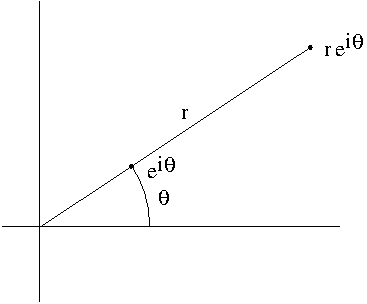
\includegraphics[height=1.5in]{5_complexpolar}}
\caption{Polar representation of a complex number.
\label{fig_complexpolar}}
\end{figure}

Notice that $r$ is exactly the length (sometimes called the modulus)
of the complex number $re^{i\theta}$.  The angle $\theta$ is called the argument. This
representation of complex numbers makes the definition of complex
multiplication more transparent.  We have
\[
r_1e^{i\theta_1}r_2e^{i\theta_2} = r_1r_2e^{i(\theta_1+\theta_2)}
\]

In other words, when we multiply two complex numbers, the moduli get
multiplied and the arguments get added.

\section{MATLAB}

Complex numbers are handled naturally by MATLAB.  Specifying a complex
number is done with the syntax {\tt z = 1+3i}. The commands {\tt
real(z)} and {\tt imag(z)} return the real and imaginary parts of a
complex number z. The commands {\tt abs(z)} and {\tt conj(z)} return
the length and conjugate of $z$. Typing {\tt sqrt(-1)} returns
\begin{verbatim}
ans =
        0 + 1.0000i
\end{verbatim}
MATLAB commands {\tt det}, {\tt rref}, and {\tt inv} all work on complex matrices. 

\section{Problems}

\begin{problem}
\label{op4_5}
Show that $|zw|=|z||w|$ for complex numbers $z$ and $w$.
\end{problem}

\begin{problem}
\label{op4_6}
Show that $\overline{zw}=\bar z \bar w$ for complex numbers $z$ and $w$.
\end{problem}

\begin{problem}
\label{op4_7}
Show that $z\bar z= |z|^2$ for every complex numbers $z$.
\end{problem}

\begin{problem}
\label{2009_a10_1}
Simplify the following expressions to the form $x + iy$.
\begin{enumerate}
\item $\displaystyle i(2-3i)(-2+i)$
\item $\displaystyle \frac{5}{(1-i)(2-i)(3-i)}$
\item $(-1+i)^{50}$
\end{enumerate}
\end{problem}

\begin{problem}
\label{2009_a10_2}
Prove that
\begin{enumerate}

\item $\displaystyle \left|\frac{z_1}{z_2}\right| = \frac{|z_1|}{|z_2|}$;
\item $\overline{(z^n)} = (\bar{z})^n$ for all $n \in \mathbb{N}$;
\item $\displaystyle \frac{1}{z} = \bar{z}$ if $|z| = 1$;
\item $z$ is either real or pure imaginary if $(\bar{z})^2 = z^2$.

\end{enumerate}
\end{problem}

\begin{problem}
\label{2009_a10_3}
There are three values of $z$ which gives $z^3 = -i$. Find all three values in the form $x + iy$.
\end{problem}

\section{Solutions to Chapter Problems} 

%%%%%%%%%%%%%%%%%%%%%%%%%%%%%%%%%%%%%%%%%%%%%%%%%%%%%%%%%%%%%%%%%%%%%%%%%%%%%%%%
\vspace{2mm}
\noindent {\bf Solution~\ref{op4_5}}
If $z=x+iy$ and $w=s+it$ then $zw=xs-yt +i(xt+ys)$ so $|zw|^2= (xs-yt)^2+(xt+ys)^2
=x^2s^2+y^2t^2-2xyst + x^2t^2+y^2s^2+2xyst=(x^2+y^2)(s^2+t^2)=|z|^2|w|^2$.

%%%%%%%%%%%%%%%%%%%%%%%%%%%%%%%%%%%%%%%%%%%%%%%%%%%%%%%%%%%%%%%%%%%%%%%%%%%%%%%%
\vspace{2mm}
\noindent {\bf Solution~\ref{op4_6}}
If $z=x+iy$ and $w=s+it$ then $zw=xs-yt +i(xt+ys)$ so $\overline{zw}=xs-yt -i(xt+ys)$.
On the other hand $\bar z \bar w=(x-iy)(s-it)=xs-yt -i(xt+ys)$.

%%%%%%%%%%%%%%%%%%%%%%%%%%%%%%%%%%%%%%%%%%%%%%%%%%%%%%%%%%%%%%%%%%%%%%%%%%%%%%%%
\vspace{2mm}
\noindent {\bf Solution~\ref{op4_7}}
If $z=x+iy$ then $z\bar z = (x+iy)(x-iy)=x^2+y^2=|z|^2$.

%%%%%%%%%%%%%%%%%%%%%%%%%%%%%%%%%%%%%%%%%%%%%%%%%%%%%%%%%%%%%%%%%%%%%%%%%%%%%%%%
\vspace{2mm}
\noindent {\bf Solution \ref{2009_a10_1}}
\begin{enumerate}[a)]
  \item
\begin{eqnarray*}
  i(2-3i)(-2+i)&=&(3+2i)(-2+i)\\
	&=&-6-4i+3i+2i^2\\
	&=&-8-i
\end{eqnarray*}
	\item
\begin{eqnarray*}
  \frac{5}{(1-i)(2-i)(3-i)}&=&\frac{5(1+i)(2+i)(3+i)}{(1-i)(2-i)(3-i)(1+i)(2+i)(3+i)}\\
	&=&\frac{5(1+3i)(3+i)}{2 \cdot 5 \cdot 10}\\
	&=&\frac{5(10i)}{100}=i/2
\end{eqnarray*}
	\item
\begin{eqnarray*}
(-1+i)^{50}&=&\left(\sqrt{2}e^{i\frac{3\pi}{4}}  \right)^{50}\\
&=&2^{25}e^{i\frac{75\pi}{2}}\\
&=&2^{25}e^{i\left(\frac{3\pi}{2}+36\pi\right)}\\
&=&2^{25}(-i)=-2^{25}i
\end{eqnarray*}
\end{enumerate}

%%%%%%%%%%%%%%%%%%%%%%%%%%%%%%%%%%%%%%%%%%%%%%%%%%%%%%%%%%%%%%%%%%%%%%%%%%%%%%%%
\vspace{2mm}
\noindent {\bf Solution \ref{2009_a10_2}}
\begin{enumerate}[a)]
  \item
Let $z_1=|z_1|e^{i\theta_1}$, $z_2=|z_1|e^{i\theta_2}$,
$$
\left|\frac{z_1}{z_2}\right|=\left|\frac{|z_1|e^{i\theta_1}}{|z_2|e^{i\theta_2}}\right|
=\left|\frac{|z_1|}{|z_2|}e^{i(\theta_1-\theta_2)}\right|=\frac{|z_1|}{|z_2|}
$$
Alternatively,
$$
\left|\frac{z_1}{z_2}\right|^2=\left(\frac{z_1}{z_2}\right)\overline{\left(\frac{z_1}{z_2}\right)}
=\left(\frac{z_1}{z_2}\right)\left(\frac{\overline{z_1}}{\overline{z_2}}\right) =
\frac{z_1\overline{z_1}}{z_2\overline{z_2}}=\frac{|z_1|^2}{|z_2|^2}
$$
Since $\left|\frac{z_1}{z_2}\right|>0$, $|z_1|>0$, $|z_2|>0$, we have that
$$
\left|\frac{z_1}{z_2}\right| = \frac{\left|z_1\right|}{\left|z_2\right|}
$$
	\item Let $z=re^{i\theta}$. Then
$$
z^n=r^ne^{in\theta}=r^ne^{-in\theta}=\left(re^{-i\theta}\right)^n=(\overline{z})^n
$$
	\item
If $|z|=1$, then $z=e^{i\theta}$. So
$$
\frac{1}{z}=\frac{1}{e^{i\theta}}=e^{-i\theta}=\overline{z}
$$
	\item
Let $z=x+iy$. Then
\begin{eqnarray*}
  (\overline{z})^2 = (x-iy)^2=x^2-y^2-2ixy\\
	z^2 = (x+iy)^2 = x^2 - y^2 + 2ixy.
\end{eqnarray*}
If $(\overline{z})^2=z^2$, then $x^2-y^2-2ixy = x^2 - y^2 + 2ixy$, therefore the condition is that $-2ixy = 2ixy$, that is, $xy=0$.

Hence, $(\overline{z})^2=z^2$ only when $z$ is either real or pure imaginary.
\end{enumerate}


%%%%%%%%%%%%%%%%%%%%%%%%%%%%%%%%%%%%%%%%%%%%%%%%%%%%%%%%%%%%%%%%%%%%%%%%%%%%%%%%
\vspace{2mm}
\noindent {\bf Solution \ref{2009_a10_3}}
If $z^3=-i$, then
$$
z=(-i)^{1/3}=\left(e^{i\frac{3\pi}{2}+2k\pi}\right)^{1/3}
$$

\begin{eqnarray*}
  k=0 &\Rightarrow &\left(e^{i\frac{3\pi}{2}}\right)^{1/3} = e^{i\frac{\pi}{2}}=i\\
	k=1 &\Rightarrow &\left(e^{i\frac{7\pi}{2}}\right)^{1/3} = e^{i\frac{7\pi}{6}}=\cos\frac{7\pi}{6}+i\sin\frac{7\pi}{6} = -\frac{\sqrt{3}}{2}-\frac{1}{2}i\\
  k=2 &\Rightarrow &\left(e^{i\frac{11\pi}{2}}\right)^{1/3} = e^{i\frac{11\pi}{6}}=\cos\frac{11\pi}{6}+i\sin\frac{11\pi}{6} = \frac{\sqrt{3}}{2}-\frac{1}{2}i\\
\end{eqnarray*}



